\section{Problema 2}
Resuelva la ecuación diferencial $\frac{\partial u}{\partial t}=k_{1} \frac{\partial^{2} u}{\partial x^{2}}+k_{2} \frac{\partial^{2} u}{\partial y^{2}}$, sobre el rectángulo $0<x<a$,
$0<y<b$, sujeta a las condiciones: $u(x, y, 0)=f(x, y), u(0, y, t)=0, u(a, y, t)=0$
$\frac{\partial u}{\partial y}(x, 0, t)=0, \frac{\partial u}{\partial y}(x, b, t)=0$

\begin{solution}
Se comienza planteando la representación gráfica del problema: 
\usetikzlibrary{patterns}
\begin{figure}[ht]
    \centering
   

% Pattern Info
 
\tikzset{
pattern size/.store in=\mcSize, 
pattern size = 5pt,
pattern thickness/.store in=\mcThickness, 
pattern thickness = 0.3pt,
pattern radius/.store in=\mcRadius, 
pattern radius = 1pt}
\makeatletter
\pgfutil@ifundefined{pgf@pattern@name@_8sa0p8rq6}{
\pgfdeclarepatternformonly[\mcThickness,\mcSize]{_8sa0p8rq6}
{\pgfqpoint{0pt}{0pt}}
{\pgfpoint{\mcSize+\mcThickness}{\mcSize+\mcThickness}}
{\pgfpoint{\mcSize}{\mcSize}}
{
\pgfsetcolor{\tikz@pattern@color}
\pgfsetlinewidth{\mcThickness}
\pgfpathmoveto{\pgfqpoint{0pt}{0pt}}
\pgfpathlineto{\pgfpoint{\mcSize+\mcThickness}{\mcSize+\mcThickness}}
\pgfusepath{stroke}
}}
\makeatother

% Pattern Info
 
\tikzset{
pattern size/.store in=\mcSize, 
pattern size = 5pt,
pattern thickness/.store in=\mcThickness, 
pattern thickness = 0.3pt,
pattern radius/.store in=\mcRadius, 
pattern radius = 1pt}
\makeatletter
\pgfutil@ifundefined{pgf@pattern@name@_whu02zlbn}{
\pgfdeclarepatternformonly[\mcThickness,\mcSize]{_whu02zlbn}
{\pgfqpoint{0pt}{0pt}}
{\pgfpoint{\mcSize+\mcThickness}{\mcSize+\mcThickness}}
{\pgfpoint{\mcSize}{\mcSize}}
{
\pgfsetcolor{\tikz@pattern@color}
\pgfsetlinewidth{\mcThickness}
\pgfpathmoveto{\pgfqpoint{0pt}{0pt}}
\pgfpathlineto{\pgfpoint{\mcSize+\mcThickness}{\mcSize+\mcThickness}}
\pgfusepath{stroke}
}}
\makeatother
\tikzset{every picture/.style={line width=0.75pt}} %set default line width to 0.75pt        

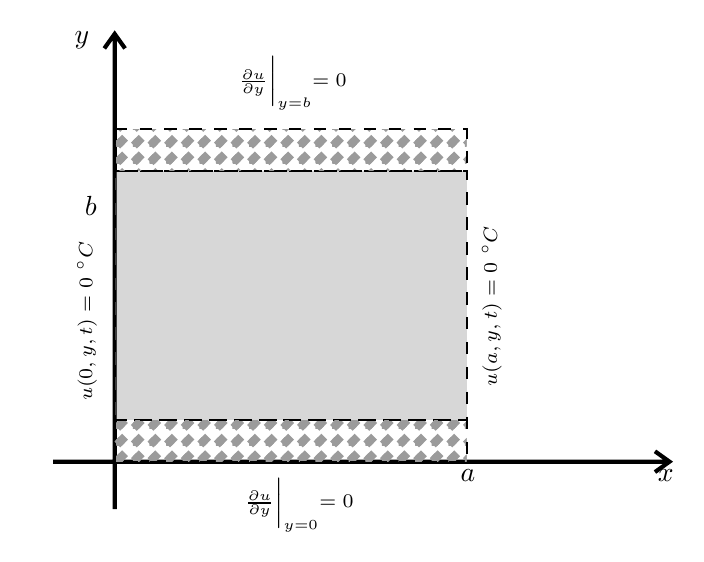
\begin{tikzpicture}[x=0.75pt,y=0.75pt,yscale=-1,xscale=1]
%uncomment if require: \path (0,300); %set diagram left start at 0, and has height of 300

%Shape: Axis 2D [id:dp8836634611392435] 
\draw [color={rgb, 255:red, 0; green, 0; blue, 0 }  ,draw opacity=1 ][line width=1.5]  (68.13,229.81) -- (365.13,229.81)(97.83,23.71) -- (97.83,252.71) (358.13,224.81) -- (365.13,229.81) -- (358.13,234.81) (92.83,30.71) -- (97.83,23.71) -- (102.83,30.71)  ;
%Shape: Rectangle [id:dp6128441923797413] 
\draw  [color={rgb, 255:red, 0; green, 0; blue, 0 }  ,draw opacity=1 ][fill={rgb, 255:red, 155; green, 155; blue, 155 }  ,fill opacity=0.4 ][dash pattern={on 4.5pt off 4.5pt}] (97.83,89.71) -- (267.43,89.71) -- (267.43,209.81) -- (97.83,209.81) -- cycle ;
%Shape: Rectangle [id:dp0645349541513307] 
\draw  [color={rgb, 255:red, 0; green, 0; blue, 0 }  ,draw opacity=1 ][pattern=_8sa0p8rq6,pattern size=6pt,pattern thickness=3pt,pattern radius=0pt, pattern color={rgb, 255:red, 155; green, 155; blue, 155}][dash pattern={on 4.5pt off 4.5pt}] (97.83,69.71) -- (267.43,69.71) -- (267.43,89.71) -- (97.83,89.71) -- cycle ;
%Shape: Rectangle [id:dp11129610169623028] 
\draw  [color={rgb, 255:red, 0; green, 0; blue, 0 }  ,draw opacity=1 ][pattern=_whu02zlbn,pattern size=6pt,pattern thickness=3pt,pattern radius=0pt, pattern color={rgb, 255:red, 155; green, 155; blue, 155}][dash pattern={on 4.5pt off 4.5pt}] (97.83,209.81) -- (267.43,209.81) -- (267.43,229.81) -- (97.83,229.81) -- cycle ;

% Text Node
\draw (56.41,118.69) node [anchor=north west][inner sep=0.75pt]  [color={rgb, 255:red, 255; green, 255; blue, 255 }  ,opacity=1 ] [align=left] {11};
% Text Node
\draw (358,232.21) node [anchor=north west][inner sep=0.75pt]    {$x$};
% Text Node
\draw (77,21.21) node [anchor=north west][inner sep=0.75pt]    {$y$};
% Text Node
\draw (78.19,202) node [anchor=north west][inner sep=0.75pt]  [font=\scriptsize,rotate=-270.03]  {$u( 0,y,t) =0\ ^{\circ } C$};
% Text Node
\draw (263,232.21) node [anchor=north west][inner sep=0.75pt]    {$a$};
% Text Node
\draw (82,100.21) node [anchor=north west][inner sep=0.75pt]    {$b$};
% Text Node
\draw (273.19,195) node [anchor=north west][inner sep=0.75pt]  [font=\scriptsize,rotate=-270.03]  {$u( a,y,t) =0\ ^{\circ } C$};
% Text Node
\draw (156,32.21) node [anchor=north west][inner sep=0.75pt]  [font=\scriptsize]  {$\frac{\partial u}{\partial y}\Bigl|_{y=b} =0$};
% Text Node
\draw (159,235.21) node [anchor=north west][inner sep=0.75pt]  [font=\scriptsize]  {$\frac{\partial u}{\partial y}\Bigl|_{y=0} =0$};


\end{tikzpicture}
   \caption{Placa rectangular metálica}
\end{figure}

Se propone utilizar el método de separación de variables: 
$$u(x,y,t)=X(x)\cdot Y(y)\cdot T(t) =X\cdot Y \cdot T $$
Es decir, sustituyendo la ecuación diferencial se tiene: 
$$XYT'= k_1 X''YT+k_2Y''XT\implies XYT'= T(k_1 X''Y+k_2Y''X)$$
$$\implies \frac{T'}{T}= \frac{k_1X''Y+k_2Y''X}{XY}\implies\fbox{$ \frac{T'}{T}=k_1\frac{X''}{X}+k_2\frac{Y''}{Y}=-\lambda$}$$

\linea 

Ahora bien, tenemos 3 casos. Dos de ellos se generan por medio de: 
$$k_1\frac{X''}{X}+k_2\frac{Y''}{Y}=-\lambda\implies k_1\frac{X''}{X} = -k_2\frac{Y''}{Y} -\lambda = -\mu $$

\linea 

Para la primera ecuación se tiene: 
$$k_1\frac{X''}{X}=-\mu\implies k_1\frac{X''}{X}+\mu X=0 \implies \fbox{$X''+\frac{\mu}{k_1}X=0$}$$
Las condiciones de frontera son:
\begin{gather*}
    X(0)= 0, \quad X(a)=0 
\end{gather*}
Nuevamente, se sabe que $\mu/k_1<0$ y $\mu/k_1=0$, se generan soluciones triviales. Por lo que solo se considerará el caso $\mu/k_1>0$. Su solución es: 
$$X(x)=A\cos \sqrt{\frac{\mu}{k_1}} x+B\sin \sqrt{\frac{\mu}{k_1}} x$$
Aplicando las condiciones de frontera: 
$$X(0)= A = 0 $$
$$X(a)=B\sin \sqrt{\frac{\mu}{k_1}}a$$
Se propone encontrar una relación para $\sqrt{\mu/k_1}a$:
$$\sqrt{\frac{\mu}{k_1}}a = \pi n\implies\sqrt{\frac{\mu}{k_1}} = \frac{\pi n}{a} $$
Por lo que la solución general es: 
$$\fbox{$X_n(x)= \sin\frac{\pi n}{a}x, \quad n=1,2,3,...$}$$
\linea 

Para la segunda ecuación se tiene: 

$$-k_2\frac{Y''}{Y}-\lambda =-\mu\implies \frac{-k_2Y''-\lambda Y}{Y}=-\mu\implies -k_2Y''-\lambda Y+\mu Y= 0$$
$$\implies k_2Y'' +\lambda Y-\mu Y=0\implies \fbox{$Y''+\frac{(\lambda-\mu)}{k_2}Y=0$}$$
Las condiciones de frontera: 
$$\frac{\partial u}{\partial y}\Big|_{y=0}=0, \quad \frac{\partial u}{\partial y}\Big|_{y=b}=0 $$
Una vez más, notamos que se generan soluciones triviales si $\frac{(\lambda-\mu)}{k_2}=0$ y $\frac{(\lambda-\mu)}{k_2}<0$. Por lo que, $\frac{(\lambda-\mu)}{k_2}>0$ es la única opción que no genera soluciones triviales y su solución es: 
$$Y(y)= C\cos\sqrt{\frac{\lambda-\mu}{k_2}}y+D\sin\sqrt{\frac{\lambda-\mu}{k_2}}y$$
$$Y'(y)= -C\sqrt{\frac{\lambda-\mu}{k_2}}\sin\sqrt{\frac{\lambda-\mu}{k_2}}y + D\sqrt{\frac{\lambda-\mu}{k_2}}\cos \sqrt{\frac{\lambda-\mu}{k_2}}y$$
Aplicando las condiciones iniciales: 
$$Y'(0)= D =0$$
$$Y'(b)= -C\sqrt{\frac{\lambda-\mu}{k_2}}\sin\sqrt{\frac{\lambda-\mu}{k_2}}b=0$$

Se propone encontrar una relación para $\sqrt{\frac{\lambda-\mu}{k_2}}$:
$$\sqrt{\frac{\lambda-\mu}{k_2}}b=\pi m\implies\sqrt{\frac{\lambda-\mu}{k_2}}= \frac{\pi m}{b}$$

Por lo que la solución general es: 
$$Y_m(y)=\cos \frac{\pi m}{b} y,\quad m=1,2,3,...$$

\linea 

Para la tercera ecuación se tiene: 
$$\implies \frac{T'}{T}=-\lambda\implies \fbox{$T'+\lambda Y=0$}$$

Excluyendo los casos triviales en donde $\lambda<0$ y $\lambda=0$, la solución para $\lambda>0$ es: 
$$Y(y)= E e^{-\lambda y}$$
Para calcular $\lambda$ se tiene de la segunda ecuación: 
$$\sqrt{\frac{\lambda-\mu}{k_2}}= \frac{\pi m}{b}\implies \lambda - \mu = k_2\left(\frac{\pi m}{b}\right)^2 \implies \lambda = \mu +k_2\left(\frac{\pi m}{b}\right)^2$$

De la primera ecuación se tiene que $\mu= k_1\left(\frac{\pi n}{a}\right)^2$, por lo que: 
$$\lambda =k_1\left(\frac{\pi n}{a}\right)^2 +k_2\left(\frac{\pi m}{b}\right)^2 $$
Por lo tanto, la solución de la ecuación es: 
\begin{align*}
    Y_{mn}(y) =\exp\left(- \left(k_1\left(\frac{\pi n}{a}\right)^2 +k_2\left(\frac{\pi m}{b}\right)^2\right)t\right)\\
    \fbox{$Y_{mn}(y) = \exp\left(- \pi^2\left(k_1\left(\frac{ n}{a}\right)^2 +k_2\left(\frac{ m}{b}\right)^2\right)t\right)$}
\end{align*}

\linea 

Ahora bien, la solución general de $u$ para $m,n=1,2,3,...$:
\begin{align*}
    u(x,y,t)_{nm} &= X(x)\cdot Y(y)\cdot T(y)\\
             &= \sin\frac{\pi n}{a}x \cdot \cos \frac{\pi m}{b} y \cdot \exp\left(- \pi^2\left(k_1\left(\frac{ n}{a}\right)^2 +k_2\left(\frac{ m}{b}\right)^2\right)t\right)
\end{align*}

\linea 

Aplicando el principio de superposición: 
\begin{align*}
    u(x,y,t) &= \sum_{m=1}^\infty\sum_{n=1}^\infty A_{mn}u_{mn}(x,y,t)\\
    &= \sum_{m=1}^\infty\sum_{n=1}^\infty A_{mn}\sin\frac{\pi n}{a}x \cdot \cos \frac{\pi m}{b} y \cdot \exp\left(- \pi^2\left(k_1\left(\frac{ n}{a}\right)^2 +k_2\left(\frac{ m}{b}\right)^2\right)t\right)
\end{align*}

\linea 

Aplicando la condición inicial en donde $t=0$, se tiene: 
\begin{align*}
    f(x,y) &= \sum_{m=1}^\infty\sum_{n=1}^\infty A_{mn}u_{mn}(x,y,t)\\
    &= \sum_{m=1}^\infty\sum_{n=1}^\infty A_{mn}\sin\frac{\pi n}{a}x \cdot \cos \frac{\pi m}{b} y
\end{align*}

\linea 

Ahora bien, tomando como referencia la ortogonalidad de los senos  y cosenos, se propone multiplicar por $\sin (k \pi x / a) \cos (l \pi y / b)$ (considerando $l$ y $k$ como $n$ y diferenciarlos) e integrar en $x$ de 0 a $a$, y en $y$ de 0 a $b$, es decir: 
$$
\begin{aligned}
& \int_{x=0}^{a} \int_{y=0}^{b} f(x, y) \sin \left(\frac{k \pi x}{a}\right) \cos \left(\frac{l \pi y}{b}\right) d y d x \\
=& \sum_{m=1}^{\infty} \sum_{n=1}^{\infty} A_{m n} \int_{x=0}^{a} \int_{y=0}^{b} \sin \left(\frac{n \pi x}{a}\right) \sin \left(\frac{k \pi x}{a}\right) \cos \left(\frac{m \pi y}{b}\right) \cos \left(\frac{l \pi y}{b}\right) d y d x \\
=& \sum_{m=1}^{\infty} \sum_{n=1}^{\infty} A_{m n} \int_{x=0}^{a} \sin \left(\frac{n \pi x}{a}\right) \sin \left(\frac{k \pi x}{a}\right) d x \int_{y=0}^{b} \cos \left(\frac{m \pi y}{b}\right) \cos \left(\frac{l \pi y}{b}\right) d y \\
=& \sum_{m=1}^{\infty} \sum_{n=1}^{\infty} A_{m n} \frac{a}{2} \delta_{n k} \frac{b}{2} \delta_{m l} \\
=& A_{l k} \frac{ab}{4}
\end{aligned}
$$
Se tiene, entonces:
$$
A_{m n}=\frac{4}{ab} \int_{x=0}^{a} \int_{y=0}^{b} f(x, y) \sin \left(\frac{n \pi x}{a}\right) \cos \left(\frac{m \pi y}{b}\right) d y d x
$$

Finalmente, la solución: 
\begin{align*}
    u(x,y,t) &=
    \sum_{m=1}^\infty\sum_{n=1}^\infty \frac{4}{ab} \int_{x=0}^{a} \int_{y=0}^{b} f(x, y) \sin \left(\frac{n \pi x}{a}\right) \cos \left(\frac{m \pi y}{b}\right) d y d x\sin\frac{\pi n}{a}x \cdot \cos \frac{\pi m}{b} y \\ &\cdot \exp\left(- \pi^2\left(k_1\left(\frac{ n}{a}\right)^2 +k_2\left(\frac{ m}{b}\right)^2\right)t\right)
\end{align*}
\end{solution}